\chapter{驱动盒}
\begin{figure}[htbp]
\centering
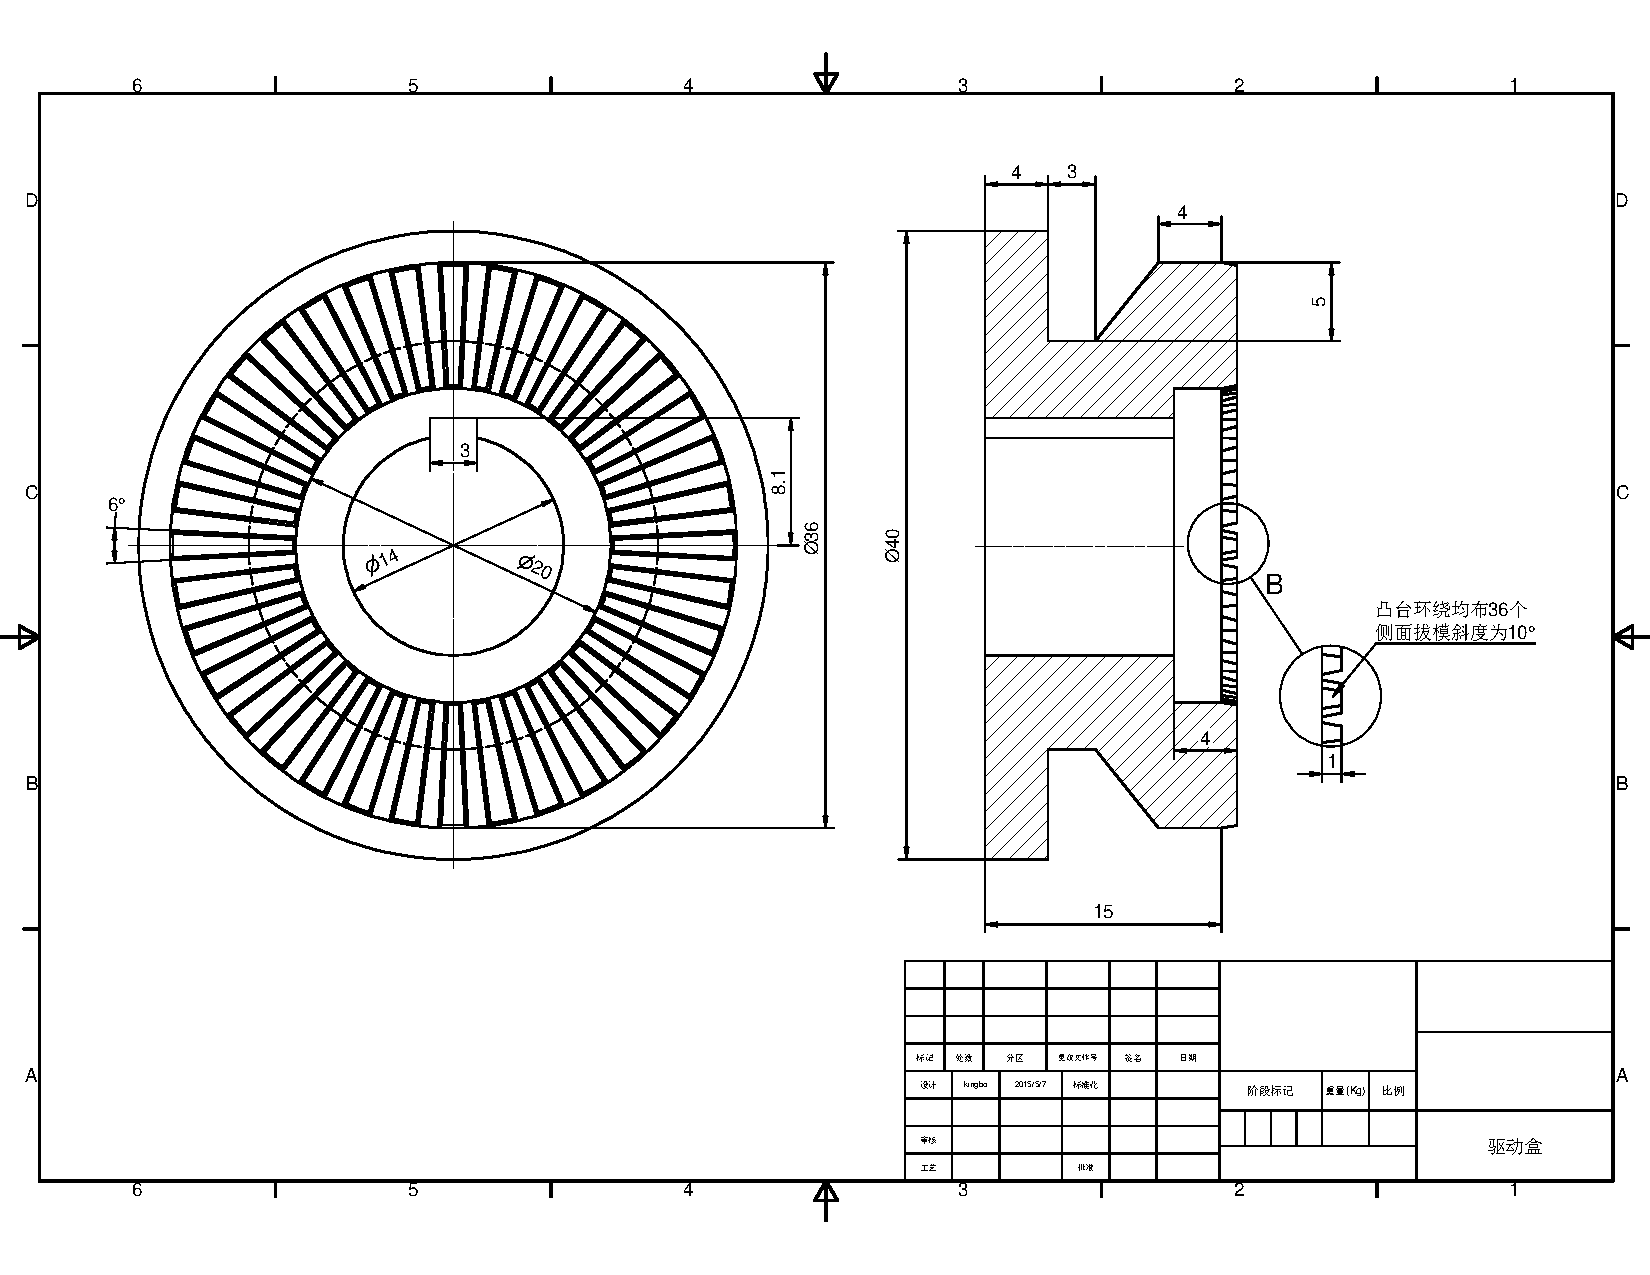
\includegraphics[scale=0.45]{qudonghe.pdf}
\caption{驱动盒零件图}\label{fig:qudonghe}
\end{figure}
%AutoCAD作为国际上广泛使用的流行的绘图工具,它具有较强的二维绘图和三维绘图功能,欢迎来到AutoCAD的三维世界,
本章我们的目标是用AutoCAD制作图\ref{fig:qudonghe}所示的航模发动机的驱动盒零件的三维模型。本章将学习以下内容:
\begin{itemize}
	\item 拉伸操作
	\item 拉伸面操作
	\item 三维对象的环形阵列操作

\end{itemize}
\endinput